\chapter{[SKE] Spolehlivostní charakteristiky, obecné rodiny hustot, cenzorování, bayesovské odhady v analýze spolehlivosti.}

Budeme pracovat s veličinou  $0\leq T\sim \FT$, která reprezentuje čas do poruchy (\textbf{Failure Time}), třeba do první chyby nebo do uzdravení pacienta. Více se však pracuje s $\RT(t)=1-\FT(t)=\PP(T>t)$ jakožto \textbf{Reliability Function}. Střední doba života (\textbf{Mean Time to Failure}) je vypočtena jako $$\MTTF:=\E T=\int_{0}^{+\infty}\big(1-\FT(t)\big)\d t - \int_{-\infty}^0\FT(t)\d t = \int_{0}^{+\infty}\RT(t)\d t=:\mu.$$

\begin{define}
	\textbf{Mediánový život} $t_\mathrm{med}$ je definován jako $\RT(t_\mathrm{med})=\frac{1}{2}$ a  \textbf{pravý krajní bod} $t_\FF$ jako  $t_\FF=\inf\{ t:\FT(t)\geq1 \}$ ($\RT$ v tomto bodě skočí na nulu a už je dále nula).
\end{define}

\begin{define}
	Intenzitu poruch (FR - \textbf{Failure Rate}) se definuje jako  $\FR(t)=\frac{f_T(t)}{\RT(t)}$.
\end{define}

Význam této veličiny je (úpravou definice) $\FR(t)=\lim\limits_{\Delta t\to 0+}\frac{1}{\Delta t}\PP(t<T\leq t+\Delta t|T>t)$, tedy že výrobek přežil do času $t$ a v následujícím $\Delta t$ čase se pokazí. Tato veličina se definuje, protože je lépe uchopitelná. Může být rostoucí i klesající. Funkce $\RT(t)$ naproti tomu je vždy klesající a pohybuje se v intervalu $[0,1]$.

\begin{theorem}[Vztahy] Platí, že
	$$ \FR(t)=\frac{-\RT(t)}{\RT(t)}=-\frac{\d}{\d t}\big(-\ln \RT(t)\big). $$
	Definujeme \textbf{Cumulative Failure Rate} jako $\Lambda_T(t):= -\ln\RT(t)$. Potom
	$$ \CFR(t) = \int_{0}^{t}\FR(u)\d u. $$
	Dále platí, že 
	$ 1-\FT(t)=\RT(t)=\e{-\CFR(t)} = \e{-\int_{0}^{t}\FR(u)\d u}$. Celkově tedy existuje jednoznačný vztah mezi $\FT$ a $\FR$ za předpokladu spojité distribuční funkce.
\end{theorem}

\begin{figure}[h]
	\centering    
	\begin{tikzpicture}
	\node[inner sep=0pt,anchor=north west] (pic) at (0,0)
	{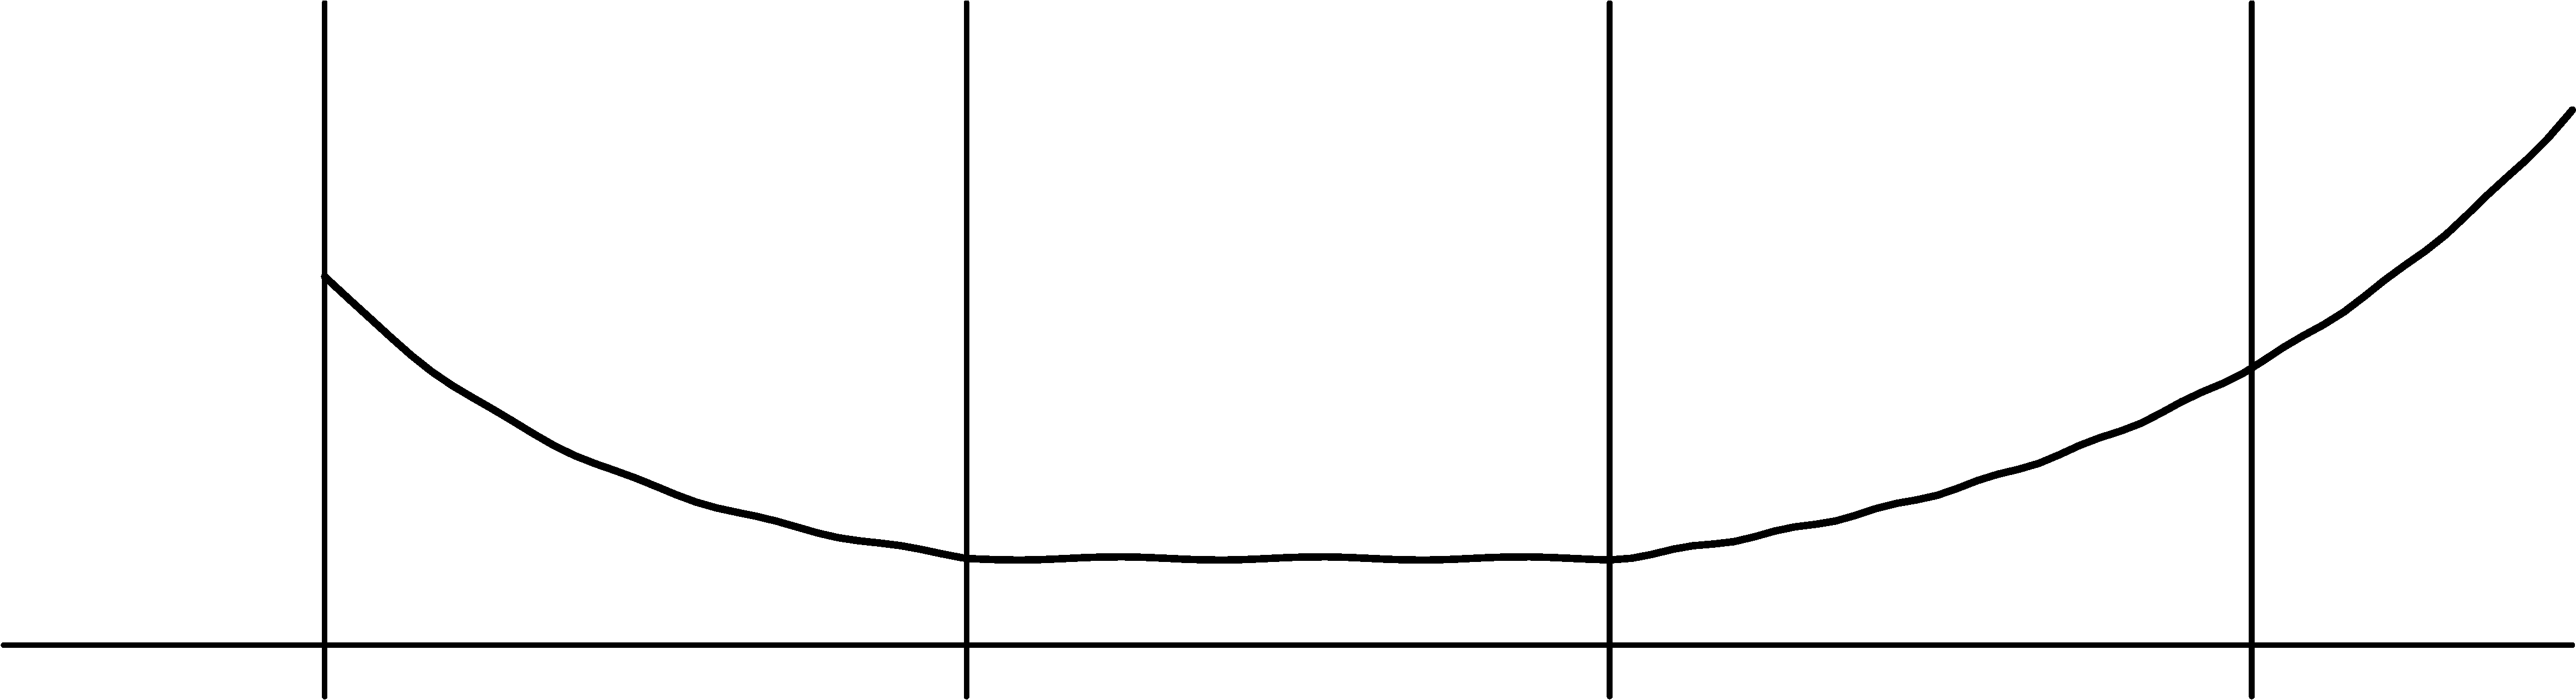
\includegraphics[width=10cm]{pictures/faze.pdf}};
	\draw [color=black](2.36,-0.2) node[anchor=north west] {I};
	\draw [color=black](4.76,-0.2) node[anchor=north west] {II};
	\draw [color=black](7.17,-0.2) node[anchor=north west] {III};
	\draw [color=black](1.3,-1.95) node[anchor=north west] {zajíždění};
	\draw [color=black](3.82,-1) node[anchor=north west] {fáze běžného};
	\draw [color=black](3.82,-1.5) node[anchor=north west] {provozu};
	\draw [color=black](7,-1.95) node[anchor=north west] {stárnutí};
	\draw [color=blue!50!black](0.72,-2.5) node[anchor=north west] {$0$};
	\draw [color=blue!50!black](9.1,-2.5) node[anchor=north west] {$t$};
	\draw [color=blue!50!black](9.2,-1) node[anchor=north west] {$\FR(t)$};
	\end{tikzpicture}
	\caption{Klasický průběh intenzity poruch (technické výrobky apod.).} \label{faze}
\end{figure}

Klasický výrobek se chová podle obr. \ref{faze}. V první fázi se vylaďují výrobní vady, a proto intenzita klesá. Ve druhé fázi je intenzita víceméně konstantní (běžný provoz). V závěrečné fázi materiál stárne a intenzita se zvyšuje.

\begin{define}
Pro $t>0$ definujeme $\RR(x|t):=\PP(T>t+x|T>t)=\frac{\RT(t+x)}{\RT(t)}$ jako \textbf{podmíněná spolehlivost}.	
\end{define}

\begin{define}
Definujeme \textbf{mean residual life} jako $$\MRL(t)=\mu(t)=\int_{0}^{+\infty}\RR(x|t)\d x=\frac{1}{\RT(t)}\int_{t}^{+\infty}\RT(u)\d u.$$
\end{define}

\begin{define}
	Pro $t_2>t_1>0$ definujeme $\RR(t_1,t_2):=\PP(T>t_2|T>t_1)$ jako \textbf{intervalovou spolehlivost}.
\end{define}

\section{Rodiny spolehlivostních modelů}
\begin{define}
	Zavádíme rodinu spolehlivostních modelů \textbf{IFR} (Increasing FR) s rostoucí FR, pokud $\FR(t)$ je rostoucí. Obecněji (pokud by nebyla k dispozici hustota) pak pokud je $\CFR$ konvexní.
	
	Analogicky naopak zavádíme \textbf{DFR} (Decreasing FR).
\end{define}

\begin{define}
	Distribuje $\FF$ je z \textbf{IFRA} rodiny (Increasing RF in Average), pokud $\frac{\CFR(t)}{t}$ je funkce rostoucí na $t>0$.
	
	Analogicky \textbf{DFRA} pro funkci klesající na $t>0$, případně $t\in(0,\t_\FF)$.
\end{define}

\begin{define}
	$\FF$ je z třídy \textbf{NBU} (New Better than Used), pokud $\RR(x|t)\leq\RR(x)=\RR(x|t=0)$, $\forall t>0,\forall x>0$. Analogicky \textbf{NWU} jako New Worse than Used.
\end{define}

\begin{define}
		$\FF$ je z třídy \textbf{NBUE} (New Better than Used in Expectation), pokud $\MRL(t)\leq \MTTF(t)$, $\forall t>0$. Analogicky \textbf{NWUE}.
\end{define}

\begin{theorem}
	$\IFR\Rightarrow\IFRA\Rightarrow\NBU\Rightarrow\NBUE$.
\end{theorem}

\section{Cenzorovaná data}
Doteď se pracovalo s úplným výběrem. Měli jsme tedy $n$ $iid$ objektů a pozorovaly se všechny časy do poruchy. Nyní se však pracuje s živými objekty (lidmi, zvířaty apod.), které se mohou rozhodnout pozorování opustit. Může se například cenzorovat časem, tj. experiment se ukončí po nějakém čase. Může se cenzorovat i počtem poruch, tj. experiment je ukončen po $r$-té poruše. Třetí možností je cenzorovat náhodně. Každý pocient je tedy cenzorován jeho vlastním cenzorovaným časem, což je náhodná veličina s $\FF_C$.

\begin{example}
	Exponenciální rozdělení $T\sim\Exp(\lambda)$ má následující vlastnosti:\begin{enumerate}
		\item $f_T(t)=\lambda\e{-\lambda t}$, $\RT(t)=\e{-\lambda t}$, $\CFR=\lambda t$, $\RR(x|t)=\e{-\lambda t}$, $\FR(t)=\lambda$
		\item $\MTTF=\frac{1}{\lambda}$, $\MRL(t)=\MTTF$
		\item celkově tedy IFR=DFR, IFRA=DFRA, NBU=NWU
	\end{enumerate}
\end{example}
\begin{theorem}[Smirnoffova transformace]
	Mějme čas do poruchy $T\sim\RT$, $\widetilde{T}:=\CFR(T)=-\ln\RT(T)$. Pak $\widetilde{T}\sim\Exp(1)$ s $\lambda_{\widetilde{T}}=1$ konstantní (tedy nestárne, ani nemládne, což vyplývá z vlastností exponenciálního času do poruchy). Navíc platí, že $T=t\Leftrightarrow \widetilde{T}=\CFR(t),~\forall t>0$ (pro spojité modely).
\end{theorem}

\section{Bayesovské odhady v analýze spolehlivosti}

\begin{define}[Gamma rozdělení]
	Mějme $T|\lambda\sim \Exp(\lambda)$ u nestabilní výroby ($\lambda=\lambda(t)$). Zde se vyplatí použít nějaké apriorní informace o $\lambda$, tedy $\lambda\sim\pi(\lambda)=\mathrm{Gamma}(k,\beta)$. Potom
	$$ \RT(t)=\int_{t}^{+\infty}f_T(u)\d u=\int_{t}^{+\infty}\int_{0}^{+\infty}\Exp(\lambda)\mathrm{Gamma}(k,\beta)\d\lambda\d u =\int_{0}^{+\infty}\mathrm{Gamma}(k,\beta)\RR_{T|\lambda}(t)\d\lambda=\frac{\beta^k}{(\beta+t)^k}, $$
	což je Paretovo rozdělení (s těžkým chvostem). Dále platí, že $\FR(t)=\frac{k}{\beta+t}$, což je klesající funkce, takže se toto rozdělení hodí např. pro modelování první fáze výrobku.
\end{define}

\begin{example}
	Jiná možnost by byla pro $(T_1...T_n)~iid~T|\lambda\sim\Exp(\lambda)$, $\lambda\sim\mathrm{Gamma}(k,\beta)$ odhadnout parametr $\lambda$ bayesovsky a dosadit ji do $\E T|\lambda$. Parametry $(k, \beta)$ lze nalézt např. pomocí empirického Bayese.
\end{example}

% lecture 5
	Užitečná je metoda pro life-time aplikace. Například k lékaři chodí v různém čase různí pacienti, takže se nabízí možnost vzít první sadu pacientů, odhadnout na ní nějaký parametr a postupně tento parametr updatujeme dalšími sadami pacientů.

Dejme tomu, že chceme udělat predikci pro $T_{n+1}$ čas do poruchy za předpokladu, že máme data $\textbf{t}=(t_1,...,t_n)$. Potom Bayesovská prediktivní spolehlivost $R_{T_{n+1}}(t):=\PP\big(T_{n+1}>t\big| t_1,...,t_n\big)=\int_{t}^{+\infty}f_\mathrm{B}^{\mathrm{PR}}(t)\d t$ se vypočítá na základě Bayesovské prediktivní hustoty ve tvaru $f_\mathrm{B}^{\mathrm{PR}}(t):=\int_{0}^{+\infty}f_T(t|\theta)\pi(\theta|\textbf{t})\d\t$. Tento způsob je sice komplikovaný, ale třeba pro měnící se $\lambda$ nejsou jiné metody k dispozici.